\chapter{Theoretical Framework}

- Cumulos globulares (definiciones, propiedades, formacion y evolucion, poblaciones estelares, etc)

\section{Globular Clusters}

Typical galaxies all around the Universe hold different structures such as stellar systems of between $ 10^{2} $ and $ 10^{6} $ stars which orbit their galactic core . We call these interesting systems star clusters and they are basically divided into two main types: Open Clusters and \textbf{Globular Clusters}.

Globular clusters are very massive stellar systems that can contain from thousands to millions of stars in a nearly spherical distribution spread over a volume of several tens to about 200 light years in diameter. These stellar systems are composed of old stars and they do not contain gas or dust. 

The average star density in a Globular Cluster is about 0.4 stars per cubic parsec. In the dense center of the cluster, the star density can increase from 100 to 1000 per cubic parsec. However, even in the center of clusters, there is still plently of space between the stars

A way of analysing globular clusters is to use Colour-Magnitude diagrams. A colour-magnitude diagram is a plot of the apparent magnitudes of the stars in a cluster against their colour indices. Globular clusters nearly all have very similar colour-magnitude diagrams

Globular clusters revolve about the nucleus of a galaxy on orbits of high eccentricity and high inclination to the galactic plane. About a third of globular clusters are concentrated around the galactic center. A typical cluster has a period of revolution around the order of $ 10^{8} $ years. A cluster spends most of its time far from the center of a galaxy, and so most of them can, and have been discovered in the spaces between galaxies.

\begin{figure}[H]
\centering
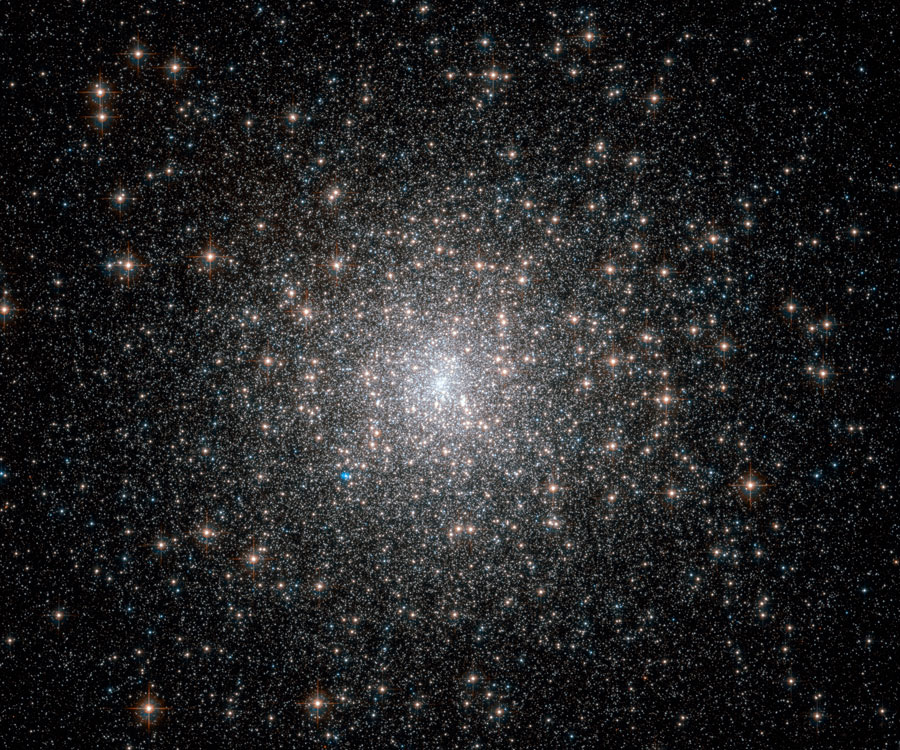
\includegraphics[width=12cm]{images/m15.jpg}
\caption{Globular Cluster M15, taken by the Hubble Space Telescope with an exposition time of 900 seconds. Image by NASA}
\end{figure}



\subsection{Photometric Properties}

\section{Stellar System Dynamics}

(we focus on globular clusters)

\subsection{Colisionless Systems}

\begin{equation}
\dfrac{df}{dt}=0
\end{equation}


\section{Scenario and Observations}

\section{Simulations}
